\documentclass[a4paper, 10pt]{article}
\usepackage[ngerman]{babel}
\usepackage[T1]{fontenc}
\usepackage[utf8]{inputenc}
\usepackage{multicol}
\usepackage{calc}
\usepackage{amsmath,amsthm,amsfonts,amssymb}
\usepackage{color,graphicx,overpic}
\usepackage{hyperref}
\usepackage{listings}
\usepackage[margin=2cm]{geometry}

\setlength{\columnsep}{.6cm}

\pdfinfo{
    /Title (CocktailShaker App - Anleitung)
    /Creator (TeX)
    /Producer (pdfTeX 3.14)
    /Author (Robert Jeutter)
    /Subject ()
}
\pagestyle{empty}
\setcounter{secnumdepth}{0}

\begin{document}
\section*{\centering 
\includegraphics[width=25px]{icon.png} CocktailShaker App - Anleitung}

\vspace{\baselineskip}

Eine kurze Anleitung anhand der unterschiedlichen Seiten der CocktailShaker App zur einfachen Übersicht aller Funktionen und Möglichkeiten.

\bigskip

\begin{multicols}{4}
    \begin{center}
        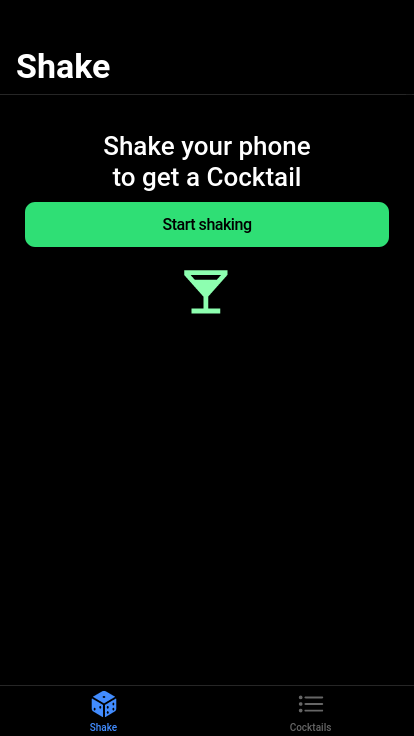
\includegraphics[width=.8\linewidth]{Start.png}
    \end{center}
    \columnbreak
    \subsection{Shake-Start}
    Der Startbildschirm ist frei und bietet die Möglichkeit, direkt zum ersten Cocktail zu schwenken oder zuerst zur Liste aller Cocktails zu wechseln. Die Navigation ist auf Shaken und Cocktailliste beschränkt.
    \columnbreak

    \begin{center}
        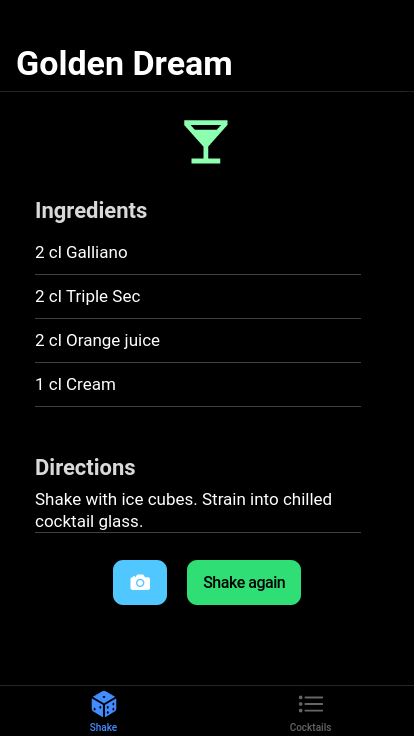
\includegraphics[width=.8\linewidth]{ShakeCocktail.png}
    \end{center}
    \columnbreak
    \subsection{Cocktail Sicht}
    Jeder Cocktail wird übersichtlich dargestellt. Ist kein Bild vorhanden, wird das zugehörige Glas als Text oder Icon angezeigt (soweit verfügbar). Über Zufall kann man ein Foto pro Cocktail hinzufügen.
\end{multicols}

\begin{multicols}{4}
    \begin{center}
        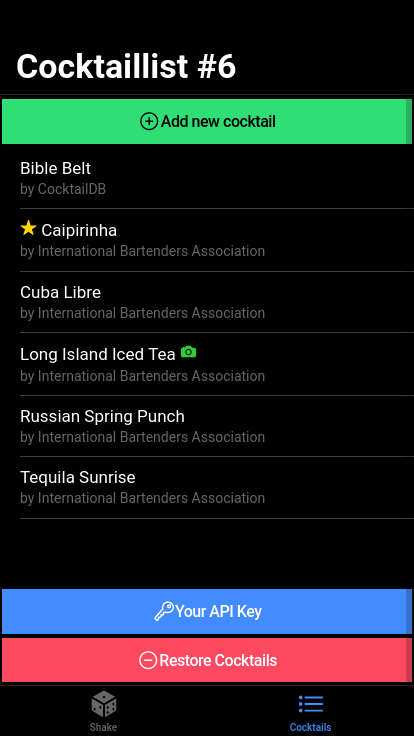
\includegraphics[width=.8\linewidth]{CocktailList-1.png}
    \end{center}
    \columnbreak
    \subsection{Cocktailliste}
    Die Liste zeigt alle gespeicherten Cocktails. Mit tippen auf den Namen gelangt man zur Cocktailsicht. Cocktails mit Kamera-Bild sind mit einem Kamerasymbol markiert.
    \columnbreak

    \begin{center}
        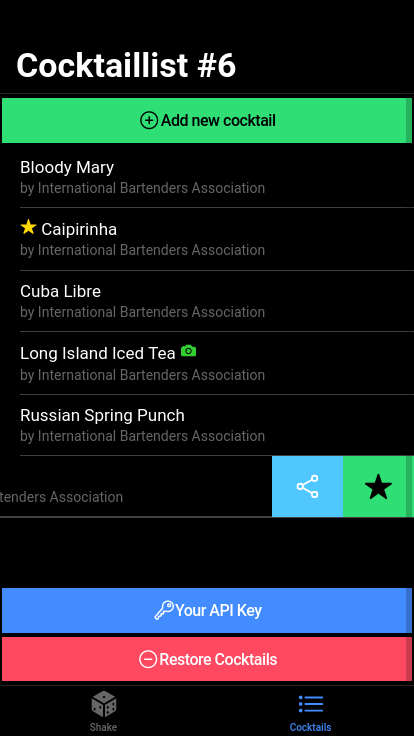
\includegraphics[width=.8\linewidth]{CocktailList-2.png}
    \end{center}
    \columnbreak
    \subsection{Cocktails Teilen und Markieren}
    Zieht man einen Cocktail nach links kann man den Cocktail favourisieren oder die Teilen-Funktion aufrufen. Favourisierte Cocktails erhalten einen Stern.
\end{multicols}

\begin{multicols}{4}
    \begin{center}
        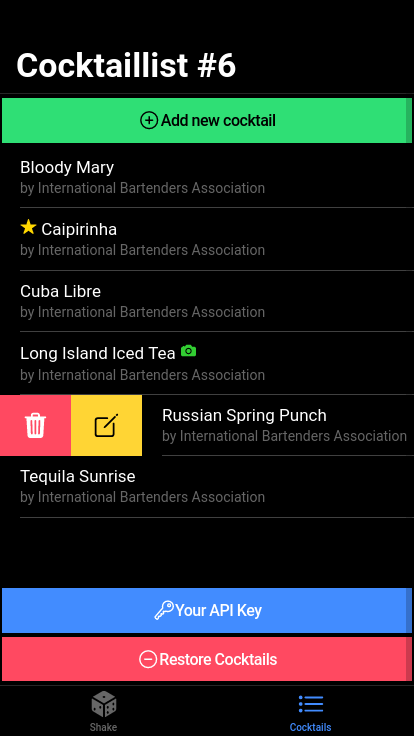
\includegraphics[width=.8\linewidth]{CocktailList-3.png}
    \end{center}
    \columnbreak
    \subsection{Cocktails bearbeiten}
    Zieht man einen Cocktail nach rechts kann man den Cocktail aus dem Smartphone löschen oder bearbeiten.
    \columnbreak

    \begin{center}
        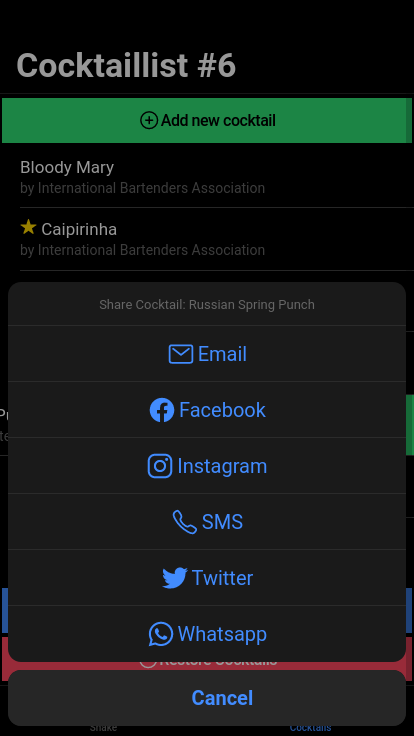
\includegraphics[width=.8\linewidth]{CocktailList-4.png}
    \end{center}
    \columnbreak
    \subsection{Cocktails teilen}
    Über die Teilen-Funktion werden Links für gängige Social-Media-Seiten erzeugt und zur Auswahl gestellt.
\end{multicols}

\begin{multicols}{4}
    \begin{center}
        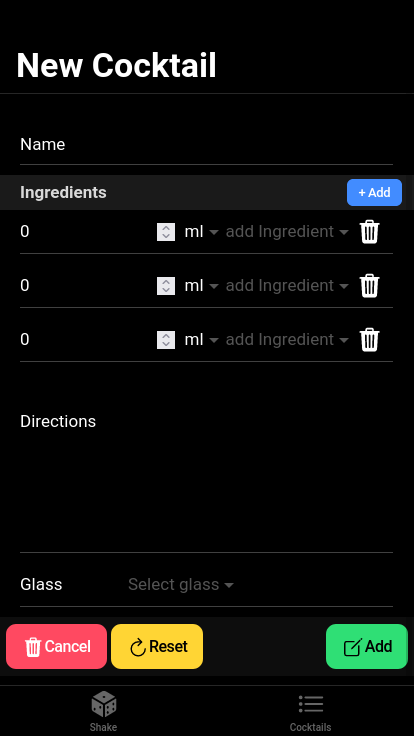
\includegraphics[width=.8\linewidth]{NewCocktail.png}
    \end{center}
    \columnbreak
    \subsection{Neue Cocktails hinzufügen}
    Neue Cocktails können hinzugefügt werden. Die Anzahl der Zutaten ist nicht beschränkt.
    \columnbreak

    \begin{center}
        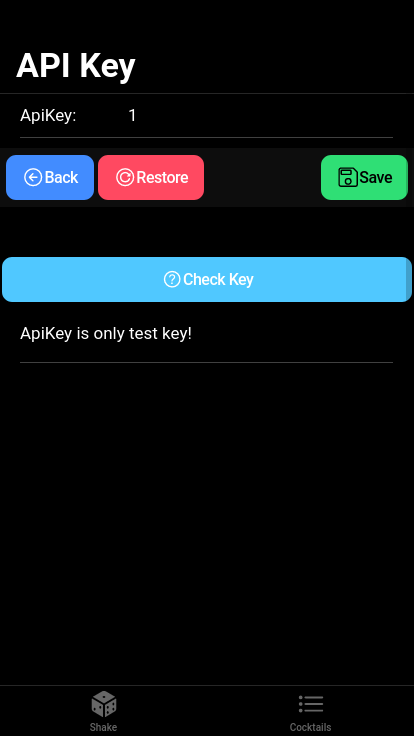
\includegraphics[width=.8\linewidth]{ApiKey.png}
    \end{center}
    \columnbreak
    \subsection{API Key ändern}
    Standardmäßig wird nur der Testkey ausgeliefert. Dieser kann hier geändert und validiert werden.
\end{multicols}

\end{document}